\documentclass[../main.tex]{subfiles}

\chapter{Our Proposal: Spoof proof atomic clock controller}\label{op}
\begin{wrapfigure}{c}{0.45\textwidth}
  \centering
  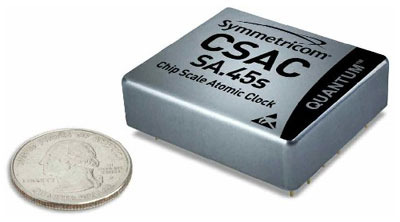
\includegraphics[width=0.40\textwidth]{csac.jpg}
  \caption[Symmetricom SA.45s CSAC]
   {Symmetricom SA.45s CSAC. Courtesy Symmetricom.}
\end{wrapfigure} 
We propose to construct and use what we call a \textit{Spoof proof atomic clock controller}. The spoof proof atomic clock controller consists of custom software running on commodity computer hardware, connected to at \textit{least} two GPS receivers and an atomic clock.
With the spoof proof atomic clock controller you can perform:
\begin{itemize}
	\item Spoofing detection.
	\begin{itemize}
		\item Having a stable clock that can be trusted makes it possible to verify the GPS timing solution. 
		\item Using two or more GPS receivers makes it possible to detect whether or not the signals originate from satellites in orbit or from a spoofer on the ground. See subsection \ref{cspakp} for more about this idea.
	\end{itemize}
	\item Mitigation.
	\begin{itemize}
		\item A stable clock will provide accurate timing for an extended time even in the absence of valid GPS correction.
	\end{itemize}
\end{itemize}

\section{Filtering and steering}
The spoof proof atomic clock controller uses what we call \textit{filters} for detection. The filters are algorithms used to detect a spoofing attack or just general abnormalities that might affect applications relying on GPS time. The filters can be divided into two classes or types. They are either GPS based or clock model based. The GPS filters analyzes collected GPS data called NMEA data \cite{NMEA_MAIN} and verifies their validity. This can be achieved by comparing the collected GPS data with known GPS data for the receivers. The clock model based filters are more sophisticated. By analyzing the behavior of the atomic clock used by the spoof proof atomic clock controller, a model can be built and used as a reference. This approach was actually suggested in subsection \ref{ctsarcs}, but in that instance using the receiver's internal clock. This approach was considered auxiliary because of the receiver's clock's poor performance. This is in contrast to our proposal where we have a stable and accurate atomic clock. This makes it possible to evaluate the GPS signal used to discipline the atomic clock. The model can also be used for mitigation during an attack. Once an attack has been detected the atomic clock should no longer be disciplined by the signal. The clock should be usable for a while without disciplining, but with the clock model used for steering it will provide accurate timing for a longer time.